\documentclass[a4paper,10pt]{scrartcl} 

\usepackage[utf8]{inputenc}     % UTF-8 Zeichensatz unter Linux -> ansonsten auf "applemac" oder "latin1" (Windows ISO-LANGE-NUMMER) ändern und diese Datei durch einen Konverter jagen ( Entsprechende Tools -> Google )
\usepackage{moreverb}
\usepackage[english]{babel}     % Deutsche Worttrennung, Umlaute etc.
\usepackage{microtype}          % Subtile Texverschönerungen
\usepackage{lmodern}            % Moderne Schrifart
\usepackage[T1]{fontenc}        % Erweiterte Textcodierung (z.B a" -> ä)
\usepackage{xcolor}             % Farbige Schrift
\usepackage{parskip}            % Absatz-Einrückung kontrollieren
\usepackage{textcomp}           % Extra Symbole (Grad Celsius etc.)
\usepackage{amssymb,amsmath}    % Schöne Formeln (AMS = American Mathematical Society)
\usepackage{graphicx}           % Bilder und Seitenränder
\usepackage{etoolbox}
\usepackage{subcaption}			% captions for subfigures
\usepackage{booktabs}           % Schönere Tabellen
\usepackage{colortbl}           % Farbige Tabellen
\usepackage[linkbordercolor={0.91 0.3 0.24},citebordercolor={0.18 0.8 0.44},urlbordercolor={0.61 0.35 0.71}]{hyperref}       % Hyperlinks im pdf
\usepackage[all]{hypcap}        % Verhaltenskorrektur für hyperref
\usepackage{url}				% URLs
\usepackage{multirow}			% Tabellen mit mehreren Einträgen/Zeile
\usepackage{tcolorbox}			% schöne bunte Boxen
\usepackage{mathtools}			% \mathclap für ordentliche \underbrace-			environments
\usepackage{geometry}			% Pagelayout mit \newgeometry, \restoregeometry
\usepackage{float}
\usepackage{wrapfig}
\usepackage{sidecap}			% side captions für Bilder; Befehl: % \begin{SCfigure}
\usepackage{bbm}				% for unity matrix (doublestroke 1) 
\usepackage{pifont}
\usepackage{enumitem}
\usepackage{siunitx}			% proper SI unit typefacing
\usepackage{nicefrac}			% slanted fractions like 3/5
%===============================%
\usepackage[singlelinecheck=false, figurename=Abb., aboveskip=7pt, belowskip=0pt]{caption}
\setcapindent{0pt}				% richtet side captions ordentlich ein

%===============================%
%\bibliographystyle{dinat}       % Literaturverzeichnis nach DIN1505

% Change the itemize labels to some other symbol - needs enumitem
\setlist[itemize,3]{label=$\triangleright$}

% where to look for graphics if they're not found
\graphicspath{{./img/}}

% own colours
%purple
\definecolor{amethyst}{HTML}{9B59B6}
\definecolor{wisteria}{HTML}{8E44AD}
%blues
\definecolor{river}{HTML}{3498DB}
\definecolor{belize}{HTML}{2980B9}
%greens
\definecolor{turkis}{HTML}{1ABC9C}
\definecolor{emerald}{HTML}{2ECC71}
\definecolor{nephritis}{HTML}{27AE60}
%orangeyellow
\definecolor{sunflower}{HTML}{F1C40F}
\definecolor{myorange}{HTML}{F39C12}
%reds
\definecolor{alizarin}{HTML}{E74C3C}
\definecolor{pome}{HTML}{C0392B}
%greyscale
\definecolor{cloud}{HTML}{ECF0F1}
\definecolor{silver}{HTML}{BDC3C7}
\definecolor{concrete}{HTML}{95A5A6}
\definecolor{midnight}{HTML}{2C3E50}
\definecolor{asphalt}{HTML}{34495E}

% renew figure and table names
\addto\captionsenglish{%
  \renewcommand{\figurename}{Fig.}%
  \renewcommand{\tablename}{Tab.}
  \renewcommand{\contentsname}{Table of Contents}%
}

% figure and table names in english
\renewcaptionname{english}{\contentsname}{Table of contents}           %Table of contents
\renewcaptionname{english}{\listfigurename}{Figures}    %Figures
\renewcaptionname{english}{\listtablename}{Tables}        %Tables
\renewcaptionname{english}{\figurename}{Fig.}               %Figure
\renewcaptionname{english}{\tablename}{Tab.}                %Table
\renewcaptionname{english}{\bibname}{Literature}             %Bibliography
  \newcaptionname{english}{\lstlistlistingname}{Table of listings} %Table of listings 
  \newcaptionname{english}{\lstlistingname}{Listing}     


% own commands
% vectorial quantities as bolded letters
\newcommand*{\vA}{\mathbf{A}}
\newcommand*{\vE}{\mathbf{E}}
\newcommand*{\vd}{\mathbf{d}}
\newcommand*{\vj}{\mathbf{j}}
\newcommand*{\vk}{\mathbf{k}}
\newcommand*{\vn}{\mathbf{n}}
\newcommand*{\vp}{\mathbf{p}}
\newcommand*{\vr}{\mathbf{r}}
\newcommand*{\vu}{\mathbf{u}}
\newcommand*{\vv}{\mathbf{v}}
% -------------------------- %
\newcommand{\bracfrac}[2]{\left( \frac{#1}{#2} \right)}
\newcommand*{\Nhat}{\hat{N}}
\newcommand*{\adagger}{\hat{a}^{\dagger}}
\newcommand*{\ahat}{\hat{a}}
\newcommand*{\lst}[1]{\left\langle #1 \right|}
\newcommand*{\rst}[1]{\left| #1 \right\rangle}
\newcommand*{\projector}[2]{\rst{#1}\lst{#2}}
% primed vectors such as v'
\newcommand*{\pvec}[1]{\vec{#1}\mkern2mu\vphantom{#1}} 
\newcommand*{\dif}{\mathrm{d}}
\newcommand*{\del}{\partial}
% bra and ket brackets
\newcommand*{\la}{\left\langle}								
\newcommand*{\ra}{\right\rangle}							
\newcommand*{\cmark}{\textcolor{emerald}{\ding{51}}}
\newcommand*{\xmark}{\textcolor{alizarin}{\ding{55}}}
\newcommand*{\rcblue}{\rowcolor{river!15}}
\newcommand{\highlight}[1]{%
  \colorbox{pome!50}{$\displaystyle#1$}}

% -------------------------- %
% absolute and norm commandos

\DeclarePairedDelimiter\abs{\lvert}{\rvert}%
\DeclarePairedDelimiter\norm{\lVert}{\rVert}%

% Swap the definition of \abs* and \norm*, so that \abs
% and \norm resizes the size of the brackets, and the 
% starred version does not.

\makeatletter
\let\oldabs\abs
\def\abs{\@ifstar{\oldabs}{\oldabs*}}
%
\let\oldnorm\norm
\def\norm{\@ifstar{\oldnorm}{\oldnorm*}}
\makeatother
% -------------------------- %
% ermöglicht Zeilenvekt.
\newcount\colveccount
\newcommand*\colvec[1]{
        \global\colveccount#1
        \begin{pmatrix*}[r]
        \colvecnext
}
\def\colvecnext#1{
        #1
        \global\advance\colveccount-1
        \ifnum\colveccount>0
                \\
                \expandafter\colvecnext
        \else
                \end{pmatrix*}
        \fi
}														
% ========================== %

% bibliography style

\usepackage[numbers]{natbib} %use sort instead of cite
\bibliographystyle{unsrtnat}

%=================Title page===================%
\begin{document}

%==============================================%
%=============BEGIN OF DOCUMENT================%
%==============================================%

\begin{titlepage}
 \begin{center}
	\Large{Fortgeschrittenenpraktikum 2}
	\end{center}
	\begin{center}
	 \LARGE{\textbf{Terahertz absorption spectroscopy}}
	\end{center}
	
	\begin{center}
	report by: \\
	Marco \textsc{Canteri} \footnote{\href{mailto:marco.canteri@student.uibk.ac.at}{marco.canteri@student.uibk.ac.at}} \& \\
	Johannes \textsc{Willi} \footnote{\href{mailto:johannes.willi@student.uibk.ac.at}{johannes.willi@student.uibk.ac.at}}
	\end{center}
	
	\begin{center}
	\vspace{1cm}
	Innsbruck, \today
	\vspace{2cm}
	\end{center}
	
	\begin{center}
	\includegraphics[scale=0.4]{img/uibk} 
	\end{center}

\end{titlepage}

\begin{abstract}
\begin{center}
\textbf{Abstract}
\end{center}
We used rotational absorption spectroscopy to probe carbon monoxide and acetonitrile in the terahertz regime. By calculating the difference between absorption frequencies we calculated the rotational constant for carbon monoxide. We also look at four absorption lines in acetonitrile, but we did not calculate rotational constants because of the non-constant bond-length.
\end{abstract}

\section{Introduction}
Absorption spectroscopy is a very useful tool in determining spectra of gases and liquids via measuring absorption of light in molecules or atoms. An absorption occurs exactly when the frequency of the light matches that of a resonant transition of the medium of interest. Lasers provide the necessary narrow bandwidth/chromaticity to "hit" such transitions. The most important are
\begin{itemize}
\item \textbf{Electronic transitions:} the transition from a low electronic into a high electronic state occurs very fast and often around the range of visible light, at roughly 400 to 800 nm wavelength.
\item \textbf{Vibrational transitions:} different vibrational modes in a molecule can also be excited.
\item \textbf{Rotational transitions:} since rotation is quantised on the quantum level, we can look at absorptions via spectroscopy as well. For this we mostly need wavelengths near/under infrared, which corresponds to a frequency in the terahertz regime.
\end{itemize}

In this experiment in particular, we looked at two molecules, carbon monoxide (CO) and acetonitril (CH$_3$CN). We cannot directly produce terahertz radiation via a laser, but we can use photomixing to obtain radiation of the order of approximately 0.3 THz up to 3 THz.

\section{Theory}

\subsection{Creating terahertz radiation}

To probe the rotational transitions in our molecules, optical laser light is far too high in frequency. We can, however, create radiation in the terahertz regime we need with a terahertz antenna \cite{fp2} \footnote{If not specified explicitly otherwise, this is assumed to be our primary source.}. This is basically a semiconductor material with electrodes at the ends that uses photomixing to create the desired frequency radiation: two lasers with a frequency difference in the desired regime are superimposed and hit the semiconductor. If the energy of the lasers and the band gap of the material are similar, electrons can be transferred inside the semiconductor from the valence band into the conduction band. By applying a voltage the electrons are accelerated and current flows until the electrons recombine with holes in the valence band. By the laws of electromagnetism, accelerated charges emit radiation transverse to the direction of propagation. Tuning this process allows terahertz radiation between approximately 0.3 and 3 THz to be produced. The produced radiation can be collimated and focused through the medium.

\subsection{Lock-in amplification for noise reduction}

Lock-in amplification is an efficient technique to filter a useful signal from an otherwise noisy background. As a basis, the useful signal is modulated by a reference (in our case, a sine wave). Feeding the same frequency to the lock-in amplifier and calculating the cross correlation between use- and reference-signal for a fixed phase shift allows us to sieve out frequencies of the total signal that are not useful because the cross-correlation in this case is zero (and the amplifier then doesn't produce a output signal).
The output signal of the lock-in amplifier is then
\begin{equation}
U_\mathrm{out} (t) = \frac{1}{T} \int\limits_{t-T}^t \sin (\omega_\mathrm{ref} s + \Delta \Phi) U_\mathrm{in}(s) \dif s
\end{equation}
where $\omega_\mathrm{ref}$ is the reference signal frequency \cite{thinksrs} and $U_\mathrm{in}$ is the signal. For sufficiently large integration time $T$, a sinusoidal input signal becomes a cosine signal with the phase shift as its argument, i.e.,
\begin{equation}
U_\mathrm{out} (t) \propto U_\mathrm{in} \cos (\Delta \Phi)
\end{equation}
Then, for integer multiples of $\pi$, the output signal of the lock-in amplifier is maximized.

\subsection{Golay cell}

We do not go into very much detail about the Golay cell here. The basic principle is that the (near-)IR terahertz radiation is absorbed by the (calibrated) gas in the Golay cell. In doing so, it warms up and bulges a flexible membrane outward. An optical sensor can detect this bulge and calculate an absorption signal from it.

\subsection{Absorption lines}

The form of any absorption line is fundamentally influenced by its natural linewidth, which is governed by the Heisenberg uncertainty relation. If we look at e.g. an electronic transition, the electron spontaneously decays after a certain lifetime. This decay can be modeled by an exponential distribution, which, if Fourier transformed, yields a Lorentz profile. For a theoretical excited state with infinite lifetime, this would converge to a Dirac delta line shape.

There are, however, other mechanisms that influence the line shape, e.g. collisions or interactions with electric fields of ions. The total influence of such interactions is called pressure broadening. Collisions shorten the lifetime of excited states because they can take away energy from the molecule, thus broadening the line profile. Pressure broadening is also Lorentzian in shape.

The thermal movement of the atoms also causes another type of broadening -- Doppler broadening. If an atom/molecule moves inside the light field of the laser, it can "see" a different wavelength because of the Doppler shift. This means a transition can not only happen at exact frequencies, but also at slightly higher or lower frequencies. Since the velocity distribution of the atoms/molecules is Boltzmann-distributed, the corresponding line shape for Doppler broadening is a Gaussian.

These effects combined give a so called Voigt-profile, a convolution of Lorentz and Gauss profile. Often, this is approximated very well by a Pseudo-Voigt-profile $f_V$ that relies on superposition instead of a (computationally more expensive) convolution. Written explicitly, the function looks like this
\begin{equation}\label{eq:pseudo_voigt}
f_V = y_0 + A \left( \frac{2 \mu}{\pi} \frac{w_L}{4(x-x_c)^2 + w_L^2} + (1-\mu) \frac{\sqrt{4 \ln 2}}{\sqrt{\pi} w_G} \exp \left( -4 \frac{\ln 2}{w_G^2}(x-x_c)^2\right) \right)
\end{equation}


\subsection{Rigid rotor model for CO}
\label{subsec:rigid_rotator}

To better understand the rotational spectrum of CO, we can imagine the molecule as a rigid rotator, i.e., two masses connected by a rigid massless rod that rotate about their common center of mass. The rotational energy is then
\begin{equation}\label{eq:E_rot}
E_\mathrm{rot} = \frac{I \omega^2}{2}
\end{equation}
where $I$ is the moment of inertia and $\omega$ the angular velocity. Writing the classical angular momentum as $J=I \omega$, eq. \eqref{eq:E_rot} becomes
\begin{equation}
E_\mathrm{rot} = \frac{J^2}{2I}
\end{equation}
Now, we know from quantum mechanics that the eigenvalues of $J^2$ are $\hbar^2 J (J+1)$, with $\hbar$ the reduced Planck constant and $J=1,2,3, \dots$ so the quantum mechanical rotational energy is
\begin{equation}
E_\mathrm{rot, QM}(J) = \frac{\hbar^2}{2I}J(J+1) = BJ(J+1)
\end{equation}
where we call $B=\hbar^2/2I$ the rotational constant. To determine $B$, we need to look at $I$ in tensor form. Written explicitly,
\begin{equation}
I = \sum_i m_i \begin{bmatrix}
y_i^2 + z_i^2 & -x_i y_i & -x_i z_i \\ 
-y_i x_i & x_i^2+z_i^2 & -y_i z_i \\ 
-z_i x_i & -z_i y_i & x_i^2+y_i^2
\end{bmatrix} 
\end{equation}
where $m_i$ are the masses of the atoms (C and O) and $\vec{r}_i = (x_i, y_i, z_i)$ is the coordinate vector of each atom relative to the center of mass. Assuming the z-axis goes exactly through C and O, the coordinates of C and O are \cite{nist1}
\[
\vec{r}_C = \begin{bmatrix}
0 \\ 
0 \\ 
\SI{0.64443}{\angstrom}
\end{bmatrix} \qquad \vec{r}_O = \begin{bmatrix}
0 \\ 
0 \\ 
\SI{-0.48377}{\angstrom}
\end{bmatrix}
\]
Using the atomic masses of $m_C = 12.0107\, \mathrm{u}$ and $m_O=15.9994\, \mathrm{u}$ \cite{nist1}, we find
\[ 
I =  \begin{bmatrix}
\SI{8.73232}{\amu\angstrom^2} 	& 0 		& 0 \\ 
0 		& \SI{8.73232}{\amu\angstrom^2} 	& 0 \\ 
0 		& 0		& 0
\end{bmatrix} 
\]
which yields to the rotational constant
\[
B_{x,y} = \frac{\hbar^2}{2I_{x,y}} = \SI{3.8348 e-23}{\joule}
\]
To express this in units of $\SI{}{\centi\meter^{-1}}$, we divide our result by $100 hc$ and obtain $B' = \SI{1.93048}{\per\centi\meter}$. Experimentally, we measure the difference between two absorption peaks. Then, the difference in rotation energy is
\begin{equation}
\Delta E_\mathrm{rot} = E_\mathrm{rot, QM}(J+1) - E_\mathrm{rot, QM}(J) = 2B =  h \Delta \nu
\end{equation}
which means, after rearranging the equation,
\begin{equation}\label{eq:rot_constant_frequency}
B = \frac{h\Delta \nu}{2}
\end{equation}

\subsection{Rotation of acetonitril}

Acetonitril is a slightly more complex molecule than carbon monoxide. It consists of a "chain" N-C-C that has 3 hydrogen atoms bound to the last C, as shown in figure \ref{fig:aceto_model}.

\begin{figure}[H]
\centering
\includegraphics[width=0.6\textwidth]{img/acetonitrile_model}
\caption{Ball-and-stick model for acetonitrile. Hydrogen is white, carbon grey, and nitrogen blue. From Wikimedia Commons \cite{wiki}.}
\label{fig:aceto_model}
\end{figure}


Mechanically, this means it has the shape of a symmetric spinning top. Rotations along the x- and y-axis (assuming the z-axis goes through the chain N-C-C) have the same moment of inertia, while along the z-axis we have to consider the three hydrogen atoms. Using the same method as in the section before with data from \cite{nist2}, we obtain
\[
I = \begin{bmatrix}
\SI{54.83536}{\amu\angstrom^2} & 0 & 0 \\ 
0 & \SI{54.83536}{\amu\angstrom^2} & 0 \\ 
0 & 0 & \SI{3.16982}{\amu\angstrom^2}
\end{bmatrix} 
\]
One can see that the light hydrogen atoms do not contribute that much, but the whole molecule is just way more massive. The rotational energy is
\begin{equation}
E_\mathrm{rot} = \frac{J_x^2 + J_y^2}{2I_x} + \frac{J_z^2}{2I_z}
\end{equation}

We want to express this in terms of $J^2=J_x^2 + J_y^2 + J_z^2$, which, after a little algebra, yields
\begin{equation}
E_\mathrm{rot} = \frac{J^2}{2I_x} + \frac{J_z^2}{2} \left(\frac{1}{I_z} - \frac{1}{I_x}\right)
\end{equation}
We can again plug in the quantum mechanical eigenvalues for $J^2$, and for the squared z-component of $J$ we plug in $m^2 \hbar^2$, where $m=(-J, -J+1, \dots J-1, J)$ is called the \textit{magnetic} quantum number and obtain
\begin{equation}
E_\mathrm{rot} = \frac{\hbar^2 J(J+1)}{2I_x} + \frac{m^2\hbar^2}{2} \left(\frac{1}{I_z} - \frac{1}{I_x}\right) = B_x J(J+1) + (B_z - B_x)m^2
\end{equation}

Finally, we obtain the following values for the rotational constants of acetonitril
\begin{align*}
B_{x,y} &= \frac{\hbar^2}{2I_x}=\SI{6.10679e-24}{\joule} \\
B_z		&= \frac{\hbar^2}{I_z} =\SI{9.88787e-23}{\joule}
\end{align*}
Again, dividing by $100 hc$ gives us the rotational constant in units of wavenumbers ($\SI{}{\per\centi\meter}$)
\[
B'_x = \SI{0.30742}{\per\centi\meter} \qquad B'_z = \SI{4.97772}{\per\centi\meter}
\]
\section{Experimental setup}

\begin{figure}[H]
\centering
\includegraphics[width=0.9\textwidth]{img/setup}
\caption[caption]{Schematic setup of the experiment. Two tunable lasers are fed into and split at a fiber switcher that puts 10\% of the light into a channel switcher and a wavemeter to feedback into and stabilize the lasers. The 90\% portion is amplified and fed into a beam splitter. The two parts are used to monitor power levels via a power meter and to actually probe the gas in our probe tube via the terahertz antenna. The standard configuration is a CO line connected directly, with a valve on both in- and outflow. For the acetonitril part, a small vessel (not shown) can be opened to allow the acetonitrol to go into the probe tube. After the beam passes the probe, it hits a Golay cell, the signal of which is noise-reduced via lock-in technique and then monitored on a PC.}
\label{fig:setup}
\end{figure}

The setup of the experiment is shown in figure \ref{fig:setup}. Our two lasers can be adjusted in frequency, either through temperature or voltage. Since the frequencies are in the regime of $\SI{e14}{\hertz}$, too high for our purposes, we need to tune them such that their frequency difference is on the order of $\SI{e11}{\hertz}$. \\
Stabilization is achieved through a feedback loop that takes 10\% of the light from the fiber switch. The wavemeter is used to monitor the individual laser frequencies as well as their difference.\\
The main part of the light is sent to an amplifier and further into a 50/50 beam splitter. One half is used to monitor power, the other is sent to the terahertz antenna, where radiation with frequency equal to the laser frequency difference is produced. A function generator, connected to both the antenna and the lock-in amplifier, modulates a sine signal onto the voltage applied to the terahertz antenna.\\
The probe tube, roughly 1 m in length, allows for enough absorption to be detected even at low pressures. The Golay cell detects changes in absorption and delivers a signal that is noise-reduced via the lock-in technique and delivered to the PC where we obtain our data. 

\section{Results}

The results of our experiments are grouped in three sections: laser stability, data for carbon monoxide, and data for acetonitril CH$_3$CN.

\subsection{Laser stability \& photodiode characteristics}

First of all, we wanted to characterize the lasers we were working with. For this, we used software installed on the PC that could take data on the frequency of each laser as well as their frequency difference for statistical analysis. These histograms are shown in figure \ref{fig:laser1} to \ref{fig:laserdifference}. We fit a Gaussian curve
\begin{equation}
f_G = y_0 + A \frac{\sqrt{2}}{\sqrt{\pi} w} \exp\left( -2 \frac{(x-x_c)^2}{w^2}\right)
\end{equation}
where $y_0$ is the y-offset/baseline, $A$ the area, $w$ the width (2 standard deviations) and $x_c$ the center/expectation value of the curve. The stability can be expressed by the Full Width at Half Maximum (FWHM)
\begin{equation}
\text{FWHM} = w \sqrt{2 \ln 2}
\end{equation}
Table \ref{tab:laser} gives a summary about these values for both lasers.

\begin{figure}[H]
\centering
\includegraphics[width=0.8\textwidth]{img/laser1stab}
\caption{Stability histogram for the first laser. The "portion" referred to in the axes label is the absolute frequency value that is left after subtracting the leading digits, i.e. 351185.5 GHz}
\label{fig:laser1}
\end{figure}

\begin{figure}[H]
\centering
\includegraphics[width=0.8\textwidth]{img/laser2stab}
\caption{Stability histogram for the second laser. Due to the same axis dimension and binning size we can see that the second laser has a slightly broader profile. Again for obtaining the portion we subtracted 350839.7 GHz}
\label{fig:laser2}
\end{figure}

\begin{figure}[H]
\centering
\includegraphics[width=0.8\textwidth]{img/differencestab}
\caption{Frequency difference histogram of our lasers. Here, a slightly bigger binning is chosen. Nevertheless, we get a very clean, symmetric Gaussian with an uncertainty on the center value in the order of $\SI{e2}{\kilo\hertz}$.}
\label{fig:laserdifference}
\end{figure}

\begin{table}
\centering
\caption{Laser characteristics as measured by the wave meter. Uncertainties come from the errors of the fit function. \label{tab:laser}}
    \begin{tabular}{l|l|l|l}
    ~          & $x_c$ / MHz       & $w$ / MHz & FHWM / MHz \\ \hline
    Laser 1    & 351185502.833(5)  & 0.795(10) & 0.936(12)    \\
    Laser 2    & 350839709.347(16) & 1.176(37) & 1.385(44)    \\
    Difference & 345793.448(21)    & 1.424(48) & 1.677(57)    \\
    \end{tabular}
\end{table}


Next, we measured the photocurrent of the terahertz antenna as a function of the applied bias voltage $U_b$. The obtained data is shown in figure \ref{fig:photocurrent}.

\begin{figure}[H]
\centering
\includegraphics[width=0.8\textwidth]{img/photocurrent}
\caption{Photocurrent as function of bias voltage. A linear fit is done on our data.}
\label{fig:photocurrent}
\end{figure}

\subsection{Carbon monoxide}

For carbon monoxide, we looked a three particular rotational transitions at $\SI{345795,9899(5)}{\mega\hertz}$, $\SI{461040,7682(5)}{\mega\hertz}$ and $\SI{576267,9305(5)}{\mega\hertz}$. These literature values are all taken from the Cologne Database of Molecular Spectroscopy \cite{cdms}.\\
First, we obtained a background spectrum by completely opening the pump valve connected to the vacuum pump to have as little pressure as possible, on the order of $\SI{2,5e-2}{\milli\bar}$. Remaining molecules in the tube are most likely ambient air molecules, i.e., mostly molecular nitrogen and oxygen. Since these molecules are symmetric they do not possess an electric dipole moment and are thus not excited rotationally.\\
To obtain the data, we then pumped carbon monoxide into our probe tube after closing the outflow valve. Once we obtained sufficient pressure, we slowly released gas to obtain data at certain pressures. Figure \ref{fig:co_all} shows all measurements taken for the 345 MHz line. These measurements were usually done over a region of 100 MHz with 2 MHz steps. However, these step sizes are not always consistent and also have uncertainties attached to them, which can be seen as x-error bars in our figures.\\
From this data we concluded that we have less broadening at roughly 0.7 mbar, which is the basis pressure for the other line measurements, i.e., for the other two lines we only obtained one data set at 0.7 mbar as well as a background. The absorption spectrum for 461 MHz can be seen in figure \ref{fig:co_461}, the spectrum for 576 MHz in figure \ref{fig:co_576}.\\
All the errors were given by our software. The fit function used in this part is called a (Pseudo-)Voigt function, as defined in eq. \eqref{eq:pseudo_voigt}. 

\begin{figure}[H]
\centering
\includegraphics[width=\textwidth]{img/co_345_all}
\caption{Complete data for the 345 MHz line of CO. One can see the relatively flat background in black and the emerging peaks for higher pressures. However, if the pressure is too high, e.g. at 1.0/2.0 mbar, the peak becomes too broad due to pressure broadening, which would lead to worse results. Due to this, we made all fits at 0.7 mbar.}
\label{fig:co_all}
\end{figure}

\begin{figure}[H]
\centering
\includegraphics[width=\textwidth]{img/co_345}
\caption{Detailed look at the 345 MHz line. Here, three different fits are shown. One can see that the Gaussian fits, both without weighting the errors or instrumentally weighting them, produce fits that are not ideally suited because they are too broad. A pure Lorentzian is not shown here, but would be too narrow. Thus, a Pseudo-Voigt is fitted which, even with its odd shape, fits the data better. The $x_c$ value of 345795.142(614) is just slightly below the literature value of $\SI{345795,9899(5)}{\mega\hertz}$ within the error bars. Still, the error bars are very large for some data points and could definitely be improved, especially around the peak.}
\label{fig:co_345_detail}
\end{figure}

\begin{figure}[H]
\centering
\includegraphics[width=\textwidth]{img/co_461}
\caption{The absorption signal around 461 MHz. Here, the fit is done with a Pseudo-Voigt function. Our value of $x_c=\SI{461040,726(196)}{\mega\hertz}$ is in good agreement with the literature value of $\SI{461040,7682(5)}{\mega\hertz}$.}
\label{fig:co_461}
\end{figure}

\begin{figure}[H]
\centering
\includegraphics[width=\textwidth]{img/co_576}
\caption{The absorption signal around 576 MHz. Again, the fit is done with a Pseudo-Voigt function. Our value of $x_c=\SI{576269,539(392)}{\mega\hertz}$ is out of agreement with the literature value of $\SI{576267,9305(5)}{\mega\hertz}$ by approximately 2 MHz. Most likely there would be another data point slightly left of our peak that corresponds to the real peak value more closely.}
\label{fig:co_576}
\end{figure}
From our measurements, the summarized results are as follows: we only have agreement with the literature values for the 461 MHz line, almost agreement for the 345 MHz line, and no agreement for the 576 MHz line. As discussed already in the figure captions, smaller step sizes and tolerances (adjustable in the Labview program) could lead to potentially better data, especially considering the Voigt-fit is quite difficult to match properly.\\
With our values, we can calculate an experimental value for the rotational constant using eq. \eqref{eq:rot_constant_frequency}. 
\begin{table}[H]
\centering
    \begin{tabular}{l|ll}
    Transition    & Exp. Value $B$                         & Theo. Value $B$                 \\ \hline
    345 - 461 MHz & $\SI{1.9220894(71)
}{\per\centi\meter}$ & $\SI{1.93048}{\per\centi\meter}$ \\
    461 - 576 MHz & $\SI{1.9218097(33)}{\per\centi\meter}$  & $\SI{1.93048}{\per\centi\meter}$ \\
    \end{tabular}\caption{Experimental values for the rotational constant, calculated via two transition frequency differences, vs the theoretical value from section \ref{subsec:rigid_rotator}. The data is not in agreement with the theoretical value, but is relatively consistent for both measurements.}
\end{table}
% From these values, we can then calculate the bond length of CO. The rotational constant expressed in cm$^{-1}$ is related to the moment of inertia via
% \begin{equation}
% B = \frac{h}{8\pi^2 c I}
% \end{equation}
% and $I$ around the symmetry axis is
% \begin{equation}
% I = m_r r^2 \qquad m_r = \frac{m_C m_0}{m_C + m_O}
% \end{equation}
\subsection{Acetonitril}
Our next molecule of interest was acetonitril. Again, a background was taken for reference at approximately $\SI{5,0e-2}{\milli\bar}$ \footnote{Since we left the valve open by recommendation of our supervisor, this value was constantly changing slightly.} and three sets of data for $\num{0,15},\num{0,07}$, and $\SI{0.3}{\milli\bar}$, where our best line shape was obtained at 0.07 mbar. In figure \ref{fig:aceto_all}, we show all obtained data points, while in figure \ref{fig:aceto_detail} we show only our data for 0.07 mbar with an appropriate fit.\\
Our fit function in figure \ref{fig:aceto_detail} is a multi-peak Pseudo-Voigt function.

\begin{figure}[H]
\centering
\includegraphics[width=\textwidth]{img/aceto_all}
\caption{All data points for the acetonitril measurement one can see emerging peaks at non-background pressures, however the double peak around 367830 MHz is only clearly visible for $p=\SI{0,07}{\milli\bar}$, which is why our analysis is done only at this pressure.}
\label{fig:aceto_all}
\end{figure}

\begin{figure}[H]
\centering
\includegraphics[width=\textwidth]{img/aceto}
\caption[caption]{The absorption spectrum for pressure $p=\SI{0,07}{\milli\bar}$. While the first and second peak from the right are clearly separated, the double peak fit parameters are obviously worse.}
\label{fig:aceto_detail}
\end{figure}


The comparison of results is shown in table \ref{tab:aceto}. We see that we are not in agreement within the error for peaks 1 and 2 (from the left) and in agreement for the double peak 3 and 4. For peaks 1 and 2, this can be explained by the sparse data points around the peaks, and for peaks 3 and 4 by the large error that occurs due to the peaks being very close and, again, sparse data. This problem could be amended by scanning over the peaks with more/finer data points and smaller tolerances.

\begin{table}[H]
\centering
    \begin{tabular}{l|l}
    Literature value \cite{cdms}       & Experimental value                    \\ \hline
     $\SI{367770.5663(2)}{\mega\hertz}$ & $\SI{367771.09(21)}{\mega\hertz}$     \\
     $\SI{367805.8689(2)}{\mega\hertz}$ & $\SI{367807.62(13)}{\mega\hertz}$     \\
    $\SI{367827.0562(3)}{\mega\hertz}$ & $\SI{367827.43 \pm 1.96}{\mega\hertz}$ \\
    $\SI{367834.1196(3)}{\mega\hertz}$ & $\SI{367834.45(72)}{\mega\hertz}$     \\
    \hline
    \end{tabular}
    \caption{Comparison of literature to experimental values for the measured transitions.\label{tab:aceto}}
\end{table}


%Compared to the literature values of 
%
%$x_{c,1}=\SI{367770.5663(2)}{\mega\hertz}$, $x_{c,2}=\SI{367805.8689(2)}{\mega\hertz}$, $x_{c,3}=\SI{367827.0562(3)}{\mega\hertz}$, $x_{c,4}=\SI{367834.1196(3)}{\mega\hertz}$ \cite{cdms} for the peaks in question, we have 
%
%$x'_{c,1}=\SI{367771.09(21)}{\mega\hertz}$, $x'_{c,2}=\SI{367807.62(13)}{\mega\hertz}$, $x'_{c,3}=\SI{367827.43\pm 1.96}{\mega\hertz}$, $x'_{c,4}=\SI{367834.45(72)}{\mega\hertz}$. 
%
%From this, we conclude that XXX

\section{Summary}

In summary, we have looked at absorption spectroscopy as a tool to probe rotational transitions in molecules. For carbon monoxide, we only had agreement for the 461 MHz line, slightly missed agreement on the 345 MHz line, and have no agreement for the 576 MHz line, while for acetonitril, we we have agreement with the literature values for the "double peak" around 367830 MHz, however for the other peaks there is a small discrepancy due to the relatively large error bars on the fit function, which comes from sparse data points. 
We could further improve our results for both species of molecules by choosing a smaller scanning window with smaller step sizes to "zoom in" on an absorption peak, or by taking more measurements at different pressures that might give a clearer line shape more suitable for fitting.

\begin{thebibliography}{9}
\bibitem{fp2}
{
Steffen Spieler, Eric Endres, and Roland Wester. \textit{Terahertz Rotations-Spektroskopie}, Universität Innsbruck, Wintersemester 2017/18
}
\bibitem{thinksrs}
{
\textit{About Lock-In Amplifiers}, Stanford Research Systems, \url{http://www.thinksrs.com/downloads/
PDFs/ApplicationNotes/AboutLIAs.pdf}
}
\bibitem{nist1}
{
\textit{Listing of experimental data for CO (Carbon Monoxide)}, National Institute of Standards and Technology, \url{http://cccbdb.nist.gov/exp2.asp?casno=630080}
}
\bibitem{nist2}
{
\textit{Listing of experimental data for CH3CN (Acetonitrile)}, National Institute of Standards and Technology, \url{http://cccbdb.nist.gov/exp2.asp?casno=75058}
}
\bibitem{wiki}
{
\textit{Acetonitrile 3-D Ball model}, \url{https://commons.wikimedia.org/wiki/File:Acetonitrile-3D-balls.png}
}
\bibitem{cdms}
{
C. P. Endres, S. Schlemmer, P. Schilke, J. Stutzki, and H. S. P. Müller,
\textit{The Cologne Database for Molecular Spectroscopy, CDMS, in the Virtual Atomic and Molecular Data Centre, VAMDC}
J. Mol. Spectrosc. 327, 95–104 (2016)
}
\end{thebibliography}

\end{document}
